\section{Activating an additional output role}
\label{sec:activation}

The channel construction supplies independent spatial outputs even after
the averaging length has been selected. We now use that independence to
eliminate the nonzero correlation supplied by Proposition~\ref{prop:selectors}.
The argument counts how many of its four factors can be read from channel
outputs. After bounding this number and choosing a correlation with the
maximal number of output roles, we take an extension that stabilizes
certain conditional expectations. This will permit a correlation with
one additional output role, contradicting maximality.

Throughout this section the selectors, and hence the assignment
$Y\mapsto\lambda_Y$, are fixed. For a channel $Y$, write $d_Y(y)$ for
its full list of spatial outputs and $x_Y(y)$ for the spatial coordinate
of its factor $\pi_Y(y)\in C$. If the output list has length $m$, its
spatial product law is $\mu^{\otimes m}$; when $m=0$ this is the
one-point probability space. All functions used below are real and
bounded.

\subsection{Correlations and an upper bound on output roles}

For $A\subseteq I$, consider a correlation
\begin{equation}\label{eq:role-correlation}
 \int \Phi(P)\prod_{i\in A}h_i(d_Y(y_i))
                  \prod_{i\notin A}h_i(x_Y(y_i))\,\dd\lambda_Y,
 \qquad P=(\omega_Y(y_i))_{i\in I}.
\end{equation}
Here $\Phi$ is an arbitrary bounded measurable function of the complete
distal parameter array. Each $h_i$ is centred for its spatial law:
$\mu^{\otimes m}$ when $i\in A$ and $\mu$ otherwise. We call the
indices in $A$ the \emph{output roles}. The functions in an output role
may depend jointly on the whole output list. Lemma~\ref{lem:channel-distal}
implies that every factor in \eqref{eq:role-correlation} is also centred
conditionally on its own parameter $P_i$.

The channel with no outputs is permitted by Definition~\ref{def:channel}.
The phase test in Proposition~\ref{prop:selectors} is measurable in the
distal parameters of the suspension. Thus that proposition gives a
nonzero correlation \eqref{eq:role-correlation} with $A=\varnothing$.
Consequently, under the supposition of pointwise failure, there is a
largest number $r\in\{0,1,2,3,4\}$ of output roles in any nonzero
correlation of this form, over all channels and all such tests.

\begin{proposition}\label{prop:role-bound}
Every nonzero correlation \eqref{eq:role-correlation} has at most two
output roles. In particular, the maximal number $r$ just defined
satisfies $r\le2$.
\end{proposition}

\begin{proof}
Apply Proposition~\ref{prop:channel-closure} to $Y$, with any
normalizing slot $b$. In the channel $\mathsf M_b(Y)$, all the copied
outputs from its four slots have their spatial product law. This
continues to hold conditionally on the old parameter array $P$, by
Corollary~\ref{cor:channel-array-distal}. This makes
\eqref{eq:role-correlation} zero
when $|A|=4$.

Suppose now that $|A|=3$, and let $b$ be the remaining slot. Starting
with $Y_0=Y$, define
\[
 Y_{n+1}=\mathsf M_b(Y_n),\qquad n\ge0,
\]
using at each step the outputs and group assignment in
Proposition~\ref{prop:channel-closure}. The state of $Y_n$ is an array
of $Y$-states indexed by $I^n$. The projection to slot $b$ at each new
axis respects the flows, since that slot has speed $b/b=1$.

In this array, consider the $n$ coordinate lines through the corner
$(b,\ldots,b)$. Each line has law $\lambda_Y$. To check this without
any symmetry assertion, first fix all but one coordinate at $b$.
Projection along a coordinate fixed at $b$ is an equivariant factor
map. If the remaining coordinate is the newly added one, functoriality
of the selected law projects it to $\lambda_Y$; if it is an earlier
coordinate, the new slot-$b$ marginal is the preceding array law.
Induction proves the assertion for every line.

All spatial output lists throughout the array are independent
conditionally on its full array of old $W_Y$-parameters, again by
Corollary~\ref{cor:channel-array-distal}. Write
$(y_i^{(a)})_{i\in I}$ for coordinate line $a$ and
$P^{(a)}=(\omega_Y(y_i^{(a)}))_i$ for its parameter array. Put
\[
 H_a=\Phi(P^{(a)})\prod_{i\ne b}h_i(d_Y(y_i^{(a)})).
\]
The products for two different lines use disjoint output lists, since
neither uses the common corner. Conditional independence and centring
give $\E[H_aH_{a'}]=0$ for $a\ne a'$. Also $\norm{H_a}_2\le K$ for a
constant $K$ depending only on the fixed tests. If
$H=h_b(x_Y(\text{corner}))$ and $c\ne0$ is the original correlation,
the line-marginal identity gives $\ip{H}{H_a}=c$ for every $a$.
Bessel's inequality therefore yields
\[
 n|c|^2\le K^2\norm H_2^2.
\]
As $n$ is arbitrary, this is impossible.
\end{proof}

\subsection{Stabilizing conditional expectations under extension}

The next extension construction prevents extra information in a later
system from changing the conditional laws that we shall use. It is an
energy-increment construction of the kind used for sated extensions
\cite[Theorem~3.11 and Lemma~3.12]{Austin}; we give the argument for the selected-law assignment
needed here.

On $(Y^I,\lambda_Y)$ introduce the five sigma-algebras
\begin{equation}\label{eq:saturation-data}
 \mathcal D_0(Y)=\sigma(P),\qquad
 \mathcal D_l(Y)=\sigma\bigl(P,(y_i)_{i\ne l}\bigr),\quad l\in I.
\end{equation}
If $\rho:Y'\to Y$ is an extension over $C$, functoriality gives the
factor map $\rho^I:(Y'^I,\lambda_{Y'})\to(Y^I,\lambda_Y)$.
The pullback of each $\mathcal D_l(Y)$ is contained in
$\mathcal D_l(Y')$, since the old distal factor is contained in the
new one.

\begin{proposition}\label{prop:saturation}
Every standard flow over $C$ has a standard extension $Y$ with the
following property. For every further standard extension
$\rho:Y'\to Y$ over $C$, every $f\in L^2(\lambda_Y)$, and every
$l\in\{0\}\cup I$,
\begin{equation}\label{eq:saturation-identity}
 \E_{\lambda_{Y'}}[f\circ\rho^I\mid\mathcal D_l(Y')]
 =\E_{\lambda_Y}[f\mid\mathcal D_l(Y)]\circ\rho^I.
\end{equation}
If the initial flow is a channel, the extension is a channel with the
same outputs pulled back to it.
\end{proposition}

\begin{proof}
For a test $f$ on a selected joining and a datum type $l$, call
\[
 \bigl\|\E[f\mid\mathcal D_l]\bigr\|_2^2
\]
its energy. Under extensions this number increases and remains bounded
by $\norm f_2^2$. Starting from the given system $Y_0$, build a sequence
of extensions $Y_0\leftarrow Y_1\leftarrow\cdots$. At each stage
introduce a countable dense subset of the
new selected joining's $L^2$ space and retain all previously introduced
tests by pullback. Schedule every retained test and every datum type
infinitely often, with positive tolerances tending to zero. At a
scheduled step, take an extension whose energy is within the prescribed
tolerance of the supremum over all standard extensions of the present
system. Such an extension exists by the definition of a supremum.

Let $Y$ be the countable inverse limit. It is a standard flow over $C$.
By Proposition~\ref{prop:selected}, its selected law projects to all
the stage laws. The union of the stage $L^2$ spaces is dense in
$L^2(\lambda_Y)$: the sigma-algebra on the fourfold inverse limit is
generated by its stage coordinate factors.

Fix a retained test $f$, a datum type $l$, and an extension $Y'$ of
$Y$. If stage $n+1$ optimized this pair with error $\epsilon_n$, then
$Y'$ is also an extension available over stage $n$. Hence
\begin{align*}
 \operatorname{energy}_{Y'}(f)
 &\le\sup_{R\to Y_n}\operatorname{energy}_{R}(f)\\
 &\le\operatorname{energy}_{Y_{n+1}}(f)+\epsilon_n
 \le\operatorname{energy}_{Y}(f)+\epsilon_n.
\end{align*}
Along the scheduled subsequence $\epsilon_n\to0$. Monotonicity gives
the opposite inequality, so the two energies are equal. The old
conditional-expectation subspace is contained in the new one; equality
of the two projection norms therefore implies equality of the
projections. This proves \eqref{eq:saturation-identity} for the retained
tests. Conditional expectation is an $L^2$ contraction, so density
proves it for every $f\in L^2(\lambda_Y)$.

This argument uses only inclusion of the datum spaces under extension;
it does not require an inverse-limit identity for maximal distal
factors. Finally, Lemma~\ref{lem:channel-distal} shows that retaining
the outputs makes every stage and the limit a channel.
\end{proof}

We call a system satisfying Proposition~\ref{prop:saturation}
\emph{saturated}. A nonzero correlation persists under the passage to
a saturated extension: its functions pull back, and its old parameter
test remains measurable in the enlarged distal parameters.

\subsection{A channel carrying the three other factors}

Choose a nonzero correlation with the maximal number $r$ of output
roles, and replace its channel by a saturated extension $Y$. Retain
the notation $A,\Phi,h_i$ for its tests. Proposition~\ref{prop:role-bound}
gives $r\le2$, so choose $b\in I\setminus A$. Set
\[
 Z=\mathsf M_b(Y),\qquad Z\longrightarrow Y,\quad
 (y_j)_{j\in I}\longmapsto y_b.
\]
Its state law is $\lambda_Y$. We give $Z$ a new channel structure
adapted to this particular correlation. Keep the full old output list
from slot $b$, and for every $j\ne b$ add the list
\begin{equation}\label{eq:added-output-lists}
 Q_j=
 \begin{cases}
   d_Y(y_j),&j\in A,\\
   x_Y(y_j),&j\notin A,
 \end{cases}
\end{equation}
where in the second case the actual flow factor added is the copy of
$C$ in that slot. Index the new three groups by $j\in I\setminus\{b\}$.
Put $Q_j$ in group $j$ and assign the three old groups from slot $b$
bijectively to these new groups. All speeds are positive rationals.

\begin{lemma}\label{lem:regrouped-channel}
With these outputs and groups, $Z$ is a channel over its slot-$b$
copy of $C$.
\end{lemma}

\begin{proof}
Condition first on the entire old parameter array $P$ in $\lambda_Y$.
The full output collection consists of one list at each slot: $Q_j$
at $j\ne b$, and the old list $d_Y(y_b)$ at $b$. Every proper collection
of these slot lists has its spatial product law by
Proposition~\ref{prop:selected} and Lemma~\ref{lem:channel-distal}.
To verify the full product law, test by a product of one bounded spatial
function of each list and expand each function into its mean and
centred part. Every term except the all-centred term is already
determined by a proper marginal. If the all-centred conditional term
were nonzero, some bounded test of $P$ would have nonzero integral
against it. This would be a correlation \eqref{eq:role-correlation}
on $Y$ with output roles $A\cup\{b\}$, contradicting maximality of $r$.
Thus the full collection has product law conditionally on $P$.

Now take a proper subset of the three new groups together with the
original spatial coordinate $x_Y(y_b)$. At least one slot $j\ne b$ is
absent. At slot $b$, only a proper subset of the old three groups has
been retained. The conditional independence of the corresponding
proper set of slots, followed by the old channel rule at slot $b$,
gives the required spatial product law conditionally on $P$.
All phases of the new channel are functions of $P$. Integrating the
two product laws down to those phases proves the two conditions in
Definition~\ref{def:channel}.
\end{proof}

Write
\begin{equation}\label{eq:outside-product}
 q((y_j)_{j\in I})=
 \prod_{j\in A}h_j(d_Y(y_j))
 \prod_{j\notin A\cup\{b\}}h_j(x_Y(y_j)).
\end{equation}
It is a function of the three added lists $Q_j$ in a single $Z$-state.
With $y=y_b$, define
\begin{equation}\label{eq:g-and-u}
 g(P,y)=\E_{\lambda_Y}[q\mid P,y_b],\qquad
 u(e,y)=\E_{m_Z}[q\mid\omega_Z,y_b],\quad e=\omega_Z.
\end{equation}
The original nonzero correlation equals
$\E[\Phi(P)h_b(x_Y(y_b))g(P,y_b)]$, so $g$ is nonzero in $L^2$.
The two conditional expectations in \eqref{eq:g-and-u} use the same
state law, but different parameter information: $e$ contains the old
array $P$ and may contain more.

\subsection{The square and its conditional laws}

The selected law $\lambda_Z$ is a law on a square of $Y$-states.
Write $\mathbf z_i=(y_{ij})_{j\in I}$ for row $i$, a $Z$-state, and set
\[
 P_{ij}=\omega_Y(y_{ij}),\qquad
 E_i=\omega_Z(\mathbf z_i),\qquad E=(E_i)_{i\in I}.
\]
Each $E_i$ contains the complete old parameter row $(P_{ij})_j$, by
Lemma~\ref{lem:parameter-distal}. In column $b$ put
\[
 y_i=y_{ib},\qquad p=(P_{ib})_{i\in I},\qquad w=P_{bb}.
\]
Functoriality for $Z\to Y$ says that this column has law $\lambda_Y$.
Row $b$ has the same law because a single $Z$-state has law $\lambda_Y$.
Our aim is to show that
\[
 \E\bigl[q((y_i)_i)q(\mathbf z_b)\mid E\bigr]\not\equiv0.
\]
The row factor $q(\mathbf z_b)$ is read from the added outputs, so it
is the candidate for the additional output role at $b$. To establish
nonvanishing, saturation will first identify the column law given $E$
and the conditional expectation of the row factor given that column.
Figure~\ref{fig:activation-square} distinguishes these two uses of the
old selected law.

\begin{figure}[htbp]
\centering
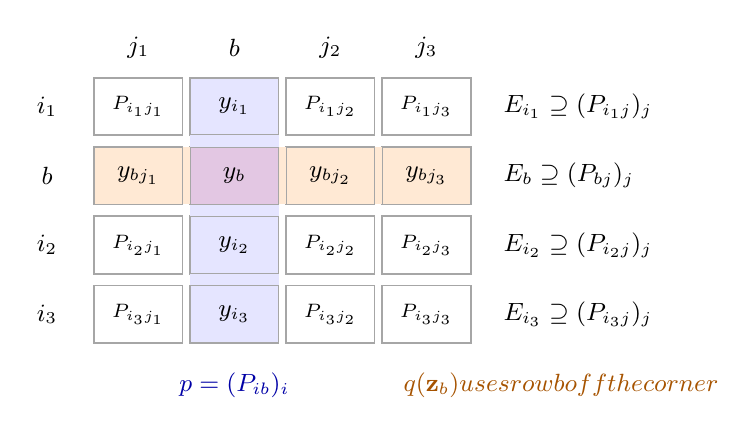
\begin{tikzpicture}[x=1.22cm,y=0.88cm,
 every node/.style={font=\small},
 cell/.style={draw=black!35,minimum width=1.13cm,minimum height=0.74cm}]
 \foreach \i in {1,2,3,4}{
   \foreach \j in {1,2,3,4}{
     \node[cell] at (\j,-\i) {};
   }
 }
 \fill[blue!10] (1.54,-4.41) rectangle (2.46,-0.59);
 \fill[orange!17] (0.54,-2.41) rectangle (4.46,-1.59);
 \fill[violet!22] (1.54,-2.41) rectangle (2.46,-1.59);
 \foreach \i in {1,2,3,4}{
   \foreach \j in {1,2,3,4}{
     \draw[black!35] (\j-0.46,-\i-0.41) rectangle
                         (\j+0.46,-\i+0.41);
   }
 }
 \node at (1,-0.15) {$j_1$};
 \node at (2,-0.15) {$b$};
 \node at (3,-0.15) {$j_2$};
 \node at (4,-0.15) {$j_3$};
 \node at (0.05,-1) {$i_1$};
 \node at (0.05,-2) {$b$};
 \node at (0.05,-3) {$i_2$};
 \node at (0.05,-4) {$i_3$};
 \node at (2,-1) {$y_{i_1}$};
 \node at (2,-2) {$y_b$};
 \node at (2,-3) {$y_{i_2}$};
 \node at (2,-4) {$y_{i_3}$};
 \node at (1,-2) {$y_{b j_1}$};
 \node at (3,-2) {$y_{b j_2}$};
 \node at (4,-2) {$y_{b j_3}$};
 \node[font=\scriptsize] at (1,-1) {$P_{i_1j_1}$};
 \node[font=\scriptsize] at (3,-1) {$P_{i_1j_2}$};
 \node[font=\scriptsize] at (4,-1) {$P_{i_1j_3}$};
 \node[font=\scriptsize] at (1,-3) {$P_{i_2j_1}$};
 \node[font=\scriptsize] at (3,-3) {$P_{i_2j_2}$};
 \node[font=\scriptsize] at (4,-3) {$P_{i_2j_3}$};
 \node[font=\scriptsize] at (1,-4) {$P_{i_3j_1}$};
 \node[font=\scriptsize] at (3,-4) {$P_{i_3j_2}$};
 \node[font=\scriptsize] at (4,-4) {$P_{i_3j_3}$};
 \node[anchor=west] at (4.7,-1) {$E_{i_1}\supseteq(P_{i_1j})_j$};
 \node[anchor=west] at (4.7,-2) {$E_b\supseteq(P_{bj})_j$};
 \node[anchor=west] at (4.7,-3) {$E_{i_2}\supseteq(P_{i_2j})_j$};
 \node[anchor=west] at (4.7,-4) {$E_{i_3}\supseteq(P_{i_3j})_j$};
 \node[blue!65!black,anchor=north] at (2,-4.7)
   {$p=(P_{ib})_i$};
 \node[orange!65!black,anchor=north] at (5.4,-4.7)
   {$q(\mathbf z_b)\text{ uses row }b\text{ off the corner}$};
\end{tikzpicture}
\caption{The square under $\lambda_Z$. Blue marks column $b$, whose
old parameter array is $p$; orange marks the row containing the added
outputs used by $q$. Their common corner has parameter $w=P_{bb}$.
The new parameters $E_i$ contain the respective old parameter rows.
The distinguished slot is drawn in second position for legibility.
The figure records marginal and factor relations, not exchangeability
of the two axes.}
\label{fig:activation-square}
\end{figure}

\begin{lemma}\label{lem:square-conditional}
In the square just defined, the conditional law of column $b$ given
$E$ is its $\lambda_Y$ law given $p$. Moreover,
\begin{equation}\label{eq:square-row-locality}
 \E_{\lambda_Z}[q(\mathbf z_b)\mid E,(y_i)_{i\in I}]
       =u(E_b,y_b).
\end{equation}
In particular, the conditional law of $y_b$ given $E$ is
$m_Y(\dd y\mid w)$; in a single $Z$-state, the conditional law of its
slot-$b$ state given $e=\omega_Z$ is the same fibre law over its old
slot-$b$ parameter.
\end{lemma}

\begin{proof}
Apply saturation of $Y$ to the extension $Z\to Y$. Under the induced
map $Z^I\to Y^I$, the old joining is precisely column $b$, and the new
datum $\mathcal D_0(Z)$ is $\sigma(E)$. Equation~\eqref{eq:saturation-identity}
for $l=0$, first on a countable determining family, gives the first
conditional-law assertion. The singleton case of
Proposition~\ref{prop:selected} then gives
\begin{equation}\label{eq:corner-fibre-law}
 \mathcal L(y_b\mid E)=m_Y(\cdot\mid w).
\end{equation}
Taking the row-$b$ marginal and applying the tower property from $E$
to its coordinate $E_b$ gives
the stated single-state assertion.

For \eqref{eq:square-row-locality}, fix $l\ne b$ and denote by
$\mathbf z_{-l}$ all rows except row $l$. Given $E$, these three rows
are independent with their $Z$ fibre laws, by
Proposition~\ref{prop:selected} applied to $Z$. In particular,
\begin{equation}\label{eq:omit-one-column-state}
 \E[q(\mathbf z_b)\mid E,(y_i)_{i\ne l}]=u(E_b,y_b).
\end{equation}
It remains to justify adding $y_l$ to the conditioning. For every
bounded measurable test $F$ of a $Y$-state, saturation for the datum
type $l$ gives
\begin{equation}\label{eq:missing-state-markov}
 \E[F(y_l)\mid E,\mathbf z_{-l}]
 =\E_{\lambda_Y}[F(y_l)\mid p,(y_i)_{i\ne l}].
\end{equation}
The right side is measurable in $(E,(y_i)_{i\ne l})$. Thus, given this
smaller datum, $y_l$ is conditionally independent of the complete rows
$\mathbf z_{-l}$. For completeness, multiplying
\eqref{eq:missing-state-markov} by any bounded function of
$\mathbf z_{-l}$ and conditioning on the smaller datum factors their
conditional product expectations. A monotone-class argument then gives
the asserted conditional independence. Since $q(\mathbf z_b)$ is
measurable in $\mathbf z_{-l}$, adjoining $y_l$ does not alter
\eqref{eq:omit-one-column-state}. This proves
\eqref{eq:square-row-locality}.
\end{proof}

We can now compute the correlation between the two highlighted lines.
First condition on the column in Lemma~\ref{lem:square-conditional},
then condition within its old law on its corner state. The result is
\begin{equation}\label{eq:square-product}
 \E\bigl[q((y_i)_i)q(\mathbf z_b)\mid E\bigr]
   =\int g(p,y)u(E_b,y)\,m_Y(\dd y\mid w).
\end{equation}
The right side is not manifestly positive. The next lemma supplies the
parameter independence that will show it cannot vanish identically.

\begin{lemma}\label{lem:parameter-reanchoring}
Under $\lambda_Z$, the variables $p$ and $E_b$ are conditionally independent
given $w=P_{bb}$.
\end{lemma}

\begin{proof}
Let $\kappa:W_Z\to W_Y$ be the factor obtained from the slot-$b$
map $Z\to Y$. This is a flow factor, and
$P_{ib}=\kappa(E_i)$. Proposition~\ref{prop:selected} identifies the
$E$ law with the ordinary deterministic-length Furstenberg law on
$W_Z$. For a bounded test $F$ of $E_b$ and a rectangle test
$\prod_i H_i(P_{ib})$, its integrated average is therefore computed
from
\[
 \int_{W_Z} F(S_{W_Z}^{bt}e)
       \prod_i H_i\bigl(\kappa(S_{W_Z}^{it}e)\bigr)\,
                         \dd m_{W_Z}(e)
\]
at each fixed $t$. Substitute $e'=S_{W_Z}^{bt}e$. The expression becomes
\[
 \int_{W_Z} F(e')
       \prod_i H_i\bigl(S_{W_Y}^{(i-b)t}\kappa(e')\bigr)\,
                         \dd m_{W_Z}(e').
\]
All factors other than $F$ depend only on $\kappa(e')$. Thus $F$ may
be replaced, at every $t$, by its conditional expectation given
$\kappa$. Averaging and taking the deterministic limit gives
\[
 \E\left[F(E_b)\prod_i H_i(P_{ib})\right]
 =\E\left[\E[F(E_b)\mid w]\prod_i H_i(P_{ib})\right].
\]
Rectangle tests generate the $p$ sigma-algebra, and $w$ is one of
its coordinates. The monotone-class theorem yields the required
conditional independence.
\end{proof}

\subsection{Nonvanishing and the additional role}

We record the elementary Hilbert-space fact used to finish the
argument. Its separability hypothesis is automatic for the probability
fibres occurring here.

\begin{lemma}\label{lem:independent-hilbert-vectors}
Let $V$ be a square-integrable random vector in a separable real
Hilbert space, and let $V'$ be an independent copy. If
$\ip V{V'}=0$ almost surely, then $V=0$ almost surely.
\end{lemma}

\begin{proof}
If $\Prob(\norm V\ge\epsilon)>0$ for some $\epsilon>0$, a countable
cover by balls of radius $\epsilon/4$ contains one ball meeting that
event with positive probability. With positive probability both $V$
and $V'$ lie in this intersection. On that event their norms are at
least $\epsilon$ and their distance at most $\epsilon/2$, so
\[
 \ip V{V'}
 =\tfrac12\bigl(\norm V^2+\norm{V'}^2-\norm{V-V'}^2\bigr)>0.
\]
This is a contradiction.
\end{proof}

\begin{proposition}\label{prop:activation}
For the saturated channel $Y$ and maximal nonzero correlation chosen
above, the regrouped channel $Z$ has a nonzero correlation
\eqref{eq:role-correlation} with output roles $A\cup\{b\}$.
\end{proposition}

\begin{proof}
We first prove that the conditional quantity in
\eqref{eq:square-product} is nonzero. In a single $Z$-state let $R(e)$
denote its old $W_Y$-parameter array; it is a function of $e=\omega_Z$.
Let $w$ denote its slot-$b$ parameter. Given $w$, write $\alpha_w$ for
the law of the old parameter array in $\lambda_Y$, and $\beta_w$ for
the law of $e$ in $m_Z$. Then $R_*\beta_w=\alpha_w$. Both old arrays,
the column array $p$ and the row array $R(E_b)$, have this same
conditional marginal. Lemma~\ref{lem:parameter-reanchoring} says that
the pair $(p,E_b)$ has conditional law $\alpha_w\otimes\beta_w$.

Work for almost every fixed $w$ in the separable real Hilbert space
$H_w=L^2(m_Y(\cdot\mid w))$. The bounded kernels
$g(p,\cdot)$ and $u(e,\cdot)$ are measurable $H_w$-valued random
vectors. To justify these assertions on a common conull set of $w$,
choose a countable generating algebra on the standard Borel space $Y$.
Its rational simple span is dense in every $H_w$; the scalar tests
against this span and Fubini give the required strong measurability.
The single-state assertion of
Lemma~\ref{lem:square-conditional} says that, conditionally on $e$,
the state $y$ has precisely the fixed law $m_Y(\cdot\mid w)$. Hence
conditioning on $R(e)$ does not introduce a $y$-dependent weight into
the distribution of $e$. The tower property for
\eqref{eq:g-and-u} gives the Hilbert-valued identity
\begin{equation}\label{eq:average-u-is-g}
 \E_{\beta_w}\bigl[u(e,\cdot)\mid R(e)\bigr]
       =g(R(e),\cdot).
\end{equation}
This can also be checked against a countable dense set in $H_w$:
the joint law of $(e,y)$ over $w$ is
$\beta_w(\dd e)m_Y(\dd y\mid w)$, and conditioning the defining
expectation of $u$ further on $(R(e),y)$ gives the defining expectation
of $g$.

Suppose now that \eqref{eq:square-product} were zero almost surely.
Conditional parameter independence would imply
\[
 \ip{g(p,\cdot)}{u(e,\cdot)}_{H_w}=0
 \quad\text{for }\alpha_w\otimes\beta_w\text{-almost every }(p,e).
\]
Average in $e$ conditionally on $R(e)$ and use
\eqref{eq:average-u-is-g}. We obtain
\[
 \ip{g(p,\cdot)}{g(p',\cdot)}_{H_w}=0
 \quad\text{for }\alpha_w\otimes\alpha_w\text{-almost every }(p,p').
\]
Lemma~\ref{lem:independent-hilbert-vectors} forces
$g(p,\cdot)=0$ almost surely for almost every $w$. This contradicts
the previously established nonvanishing of $g$.

It follows that some bounded measurable real test $\Psi(E)$ has
\begin{equation}\label{eq:activated-correlation}
 \E_{\lambda_Z}\bigl[
       \Psi(E)q((y_i)_i)q(\mathbf z_b)\bigr]\ne0.
\end{equation}
For example, take the sign of the nonzero conditional expectation
in \eqref{eq:square-product}. We identify its four roles. In every
row $i\ne b$, the factor from $q((y_i)_i)$ reads the old slot-$b$
state: when $i\in A$ it is a function of the old outputs retained in
$Z$, and when $i\notin A$ it is a function of $Z$'s original spatial
coordinate. Their spatial means remain zero. In row $b$, the factor
$q(\mathbf z_b)$ is a function of the three added lists $Q_j$.
Under the full spatial product law of the outputs of $Z$, these lists
are independent and each of its three factors is centred. Therefore
$q(\mathbf z_b)$ is itself centred for that spatial product law.
Finally $\Psi$ is a test of the full new distal parameter array $E$.
Thus \eqref{eq:activated-correlation} has exactly the form
\eqref{eq:role-correlation}, with output roles $A\cup\{b\}$, as
asserted.
\end{proof}

\begin{proof}[Proof of Theorem~\ref{thm:main}]
If the required pointwise conclusion failed, the standard coding
reduction and Proposition~\ref{prop:selectors} would supply the fixed
selectors and a nonzero correlation with no output roles. A maximal
role number $r$ would therefore exist. Proposition~\ref{prop:role-bound}
gives $r\le2$. Proposition~\ref{prop:saturation} preserves a maximal
witness in a saturated channel, and Proposition~\ref{prop:activation}
then produces a nonzero correlation with $r+1$ output roles. This
contradicts the definition of $r$. Pointwise failure is impossible.
The limiting value is the product of the four integrals, as in the
norm convergence of Lemma~\ref{lem:relative-norm}. Pulling back from
the standard coded factor proves the assertion on the original
probability space.
\end{proof}
